\documentclass[14pt,aspectratio=169]{beamer}
%%%%%%%%%%%%%%%%%%%%%%%%%%%%%%%%%%%%%%%%%%%%%%%%%%%%%%%%%%%%%
% Meta informations:
\newcommand{\trauthor}{Michael Blesel, Oliver Pola}
\newcommand{\trtype}{Seminar} %{Proseminar} %{Seminar} %{Workshop}
\newcommand{\trcourse}{Neural Networks}
\newcommand{\trtitle}{Boltzmann Machine}
\newcommand{\trmatrikelnummer}{6443269, 6769946}
\newcommand{\tremail}{\{3blesel, 5pola\}@informatik.uni-hamburg.de}
\newcommand{\trinstitute}{Dept. Informatik -- Knowledge Technology, WTM}
\newcommand{\trwebsiteordate}{{http://www.informatik.uni-hamburg.de/WTM/}}

%%%%%%%%%%%%%%%%%%%%%%%%%%%%%%%%%%%%%%%%%%%%%%%%%%%%%%%%%%%%%
% Languages:

% Falls die Ausarbeitung in Deutsch erfolgt:
% \usepackage[german]{babel}
% \usepackage[T1]{fontenc}
% \usepackage[latin1]{inputenc}
% \usepackage[latin9]{inputenc}	 				
% \selectlanguage{german}

% If the thesis is written in English:
\usepackage[english]{babel} 						
\selectlanguage{english}

%%%%%%%%%%%%%%%%%%%%%%%%%%%%%%%%%%%%%%%%%%%%%%%%%%%%%%%%%%%%%
% Bind packages:
\usepackage{beamerthemesplit}
\usetheme{Boadilla}
%\usetheme{Copenhagen}
%\usetheme{Darmstadt}
%\usetheme{Frankfurt}
%\usetheme{Ilmenau}
%\usetheme{JuanLesPins}
%\usetheme{Madrid}
%\usetheme{Warsaw }
%\usecolortheme{dolphin}
%\setbeamertemplate{sections/subsections in toc}[sections numbered]
%\beamertemplatenavigationsymbolsempty
%\setbeamertemplate{headline}[default] 	% deaktiviert die Kopfzeile
\setbeamertemplate{navigation symbols}{}% deaktiviert Navigationssymbole
%\useinnertheme{rounded}

\usepackage{acronym}                    % Acronyms
\usepackage{algorithmic}								% Algorithms and Pseudocode
\usepackage{algorithm}									% Algorithms and Pseudocode
\usepackage{amsfonts}                   % AMS Math Packet (Fonts)
\usepackage{amsmath}                    % AMS Math Packet
\usepackage{amssymb}                    % Additional mathematical symbols
\usepackage{amsthm}
\usepackage{color}                      % Enables defining of colors via \definecolor
\usepackage{fancybox}                   % Gleichungen einrahmen
\usepackage{fancyhdr}										% Paket zur schickeren der Gestaltung der 
\usepackage{graphicx}                   % Inclusion of graphics
%\usepackage{latexsym}                  % Special symbols
\usepackage{longtable}									% Allow tables over several parges
\usepackage{listings}                   % Nicer source code listings
\usepackage{lstautogobble}
\usepackage{lmodern}
\usepackage{multicol}										% Content of a table over several columns
\usepackage{multirow}										% Content of a table over several rows
\usepackage{rotating}										% Alows to rotate text and objects
\usepackage[section]{placeins}          % Ermoeglich \Floatbarrier fuer Gleitobj. 
\usepackage[hang]{subfigure}            % Allows to use multiple (partial) figures in a fig
%\usepackage[font=footnotesize,labelfont=rm]{subfig}	% Pictures in a floating environment
\usepackage{tabularx}										% Tables with fixed width but variable rows
\usepackage{url,xspace,boxedminipage}   % Accurate display of URLs

\lstset{
	frame=single,
	aboveskip=10pt,
	belowskip=10pt,
	%basicstyle={\scriptsize\ttfamily},
	basicstyle=\footnotesize,
	numbers=left,
	numberstyle=\tiny\color{gray},
	keywordstyle=\color{magenta},
	commentstyle=\color{gray},
	stringstyle=\color{teal},
	emphstyle=\color{blue},
	language=,
	breaklines=true,
	breakatwhitespace=true,
	postbreak=\hbox{$\hookrightarrow$ },
	showstringspaces=false,
	autogobble=true,
	upquote=true,
	tabsize=4,
	captionpos=b,
	morekeywords={as,with}
}

\definecolor{uhhRed}{RGB}{226,0,26}     % Official Uni Hamburg Red
\definecolor{uhhGrey}{RGB}{136,136,136} % Official Uni Hamburg Grey
\definecolor{uhhLightGrey}{RGB}{220, 220, 220}
\setbeamertemplate{itemize items}[ball]
\setbeamercolor{title}{fg=uhhRed,bg=white}
\setbeamercolor{title in head/foot}{bg=uhhRed}
\setbeamercolor{block title}{bg=uhhGrey,fg=white}
\setbeamercolor{block body}{bg=uhhLightGrey,fg=black}
\setbeamercolor{section in head/foot}{bg=black}
\setbeamercolor{frametitle}{bg=white,fg=uhhRed}
\setbeamercolor{author in head/foot}{bg=black,fg=white}
\setbeamercolor{author in footline}{bg=white,fg=black}
\setbeamercolor*{item}{fg=uhhRed}
\setbeamercolor*{section in toc}{fg=black}
\setbeamercolor*{separation line}{bg=black}
\setbeamerfont*{author in footline}{size=\scriptsize,series=\mdseries}
\setbeamerfont*{institute}{size=\footnotesize}

\newcommand{\opticalseperator}{0.0025\paperwidth}

\institute{Universit\"at Hamburg\\\trinstitute}
\title{\trtitle}
\subtitle{\trtype}
\author{\trauthor}
\date{}
\logo{}

%%%%%%%%%%%%%%%%%%%%%%%%%%%%%%%%%%%%%%%%%%%%%%%%%%%%%%%%%%%%%
% Configurationen:
%\hypersetup{pdfpagemode=FullScreen}

\hyphenation{whe-ther} 									% Manually use: "\-" in a word: Staats\-ver\-trag

%\lstloadlanguages{C}                   % Set the default language for listings
\DeclareGraphicsExtensions{.pdf,.svg,.jpg,.png,.eps} % first try pdf, then eps, png and jpg
\graphicspath{{./src/}} 								% Path to a folder where all pictures are located

%%%%%%%%%%%%%%%%%%%%%%%%%%%%
% Costom Definitions:
\setbeamertemplate{title page}
{
  \vbox{}
	\vspace{0.4cm}
  \begin{centering}
    \begin{beamercolorbox}[sep=8pt,center,colsep=-4bp]{title}
      \usebeamerfont{title}\inserttitle\par%
      \ifx\insertsubtitle\@empty%
      \else%
        \vskip0.20em%
        {\usebeamerfont{subtitle}\usebeamercolor[fg]{subtitle}\insertsubtitle\par}%
      \fi%     
    \end{beamercolorbox}%
		\vskip0.4em
    \begin{beamercolorbox}[sep=8pt,center,colsep=-4bp,rounded=true,shadow=true]{author}
      \usebeamerfont{author}\insertauthor \\ \insertinstitute
    \end{beamercolorbox}

	  \vfill
	  \begin{beamercolorbox}[ht=8ex,center]{}
		  
\includegraphics[width=0.16\paperwidth]{wtmIcon.pdf}
	  \end{beamercolorbox}%
    \begin{beamercolorbox}[sep=8pt,center,colsep=-4bp,rounded=true,shadow=true]{institute}
      \usebeamerfont{institute}\trwebsiteordate
    \end{beamercolorbox}
		\vspace{-0.1cm}
  \end{centering}
}

\setbeamertemplate{frametitle}
{
\begin{beamercolorbox}[wd=\paperwidth,ht=3.8ex,dp=1.2ex,leftskip=0pt,rightskip=4.0ex]{frametitle}%
		\usebeamerfont*{frametitle}\centerline{\insertframetitle}
	\end{beamercolorbox}
	\vspace{0.0cm}
}

\setbeamertemplate{footline}
{
  \leavevmode
	\vspace{-0.05cm}
  \hbox{
	  \begin{beamercolorbox}[wd=.32\paperwidth,ht=4.8ex,dp=2.7ex,center]{author in footline}
	    \hspace*{2ex}\usebeamerfont*{author in footline}\trauthor
	  \end{beamercolorbox}%
	  \begin{beamercolorbox}[wd=.60\paperwidth,ht=4.8ex,dp=2.7ex,center]{author in footline}
	    \usebeamerfont*{author in footline}\trtitle
	  \end{beamercolorbox}%
	  \begin{beamercolorbox}[wd=.07\paperwidth,ht=4.8ex,dp=2.7ex,center]{author in footline}
	    \usebeamerfont*{author in footline}\insertframenumber{}
	  \end{beamercolorbox}
  }
	\vspace{0.15cm}
}
\renewcommand{\footnotesize}{\fontsize{12.4pt}{12.4pt}\selectfont}
\renewcommand{\small}{\fontsize{13.8pt}{13.8pt}\selectfont}
\renewcommand{\normalsize}{\fontsize{15.15pt}{15.15pt}\selectfont}
\renewcommand{\large}{\fontsize{17.7pt}{17.7pt}\selectfont}
\renewcommand{\Large}{\fontsize{21.3pt}{21.3pt}\selectfont}

%%%%%%%%%%%%%%%%%%%%%%%%%%%%
% Additional 'theorem' and 'definition' blocks:
\newtheorem{axiom}{Axiom}[section] 	
%\newtheorem{axiom}{Fakt}[section]			% Wenn in Deutsch geschrieben wird.
%Usage:%\begin{axiom}[optional description]%Main part%\end{fakt}

%Additional types of axioms:
\newtheorem{observation}[axiom]{Observation}

%Additional types of definitions:
\theoremstyle{remark}
%\newtheorem{remark}[section]{Bemerkung} % Wenn in Deutsch geschrieben wird.
\newtheorem{remark}[section]{Remark} 

%%%%%%%%%%%%%%%%%%%%%%%%%%%%
% Provides TODOs within the margin:
\newcommand{\TODO}[1]{\marginpar{\emph{\small{{\bf TODO: } #1}}}}

%%%%%%%%%%%%%%%%%%%%%%%%%%%%
% Abbreviations and mathematical symbols
\newcommand{\modd}{\text{ mod }}
\newcommand{\RS}{\mathbb{R}}
\newcommand{\NS}{\mathbb{N}}
\newcommand{\ZS}{\mathbb{Z}}
\newcommand{\dnormal}{\mathit{N}}
\newcommand{\duniform}{\mathit{U}}

\newcommand{\erdos}{Erd\H{o}s}
\newcommand{\renyi}{-R\'{e}nyi}

%%%%%%%%%%%%%%%%%%%%%%%%%%%%
% Display of TOCs:
\AtBeginSection[]
{
	\setcounter{tocdepth}{2}  
	\frame
	{
	  \frametitle{Outline}
		\tableofcontents[currentsection]
	}
}
 
%%%%%%%%%%%%%%%%%%%%%%%%%%%%%%%%%%%%%%%%%%%%%%%%%%%%%%%%%%%%%
% Document:
\begin{document}
\renewcommand{\arraystretch}{1.2}

\begin{frame}[plain] % plain => kein Rahmen
  \titlepage
\end{frame}
%\setcounter{framenumber}{0}

\frame{
	\frametitle{Outline}
	\tableofcontents
}

\section{Boltzmann Machine}
\frame{
    \frametitle{What is a Boltzmann Machine?}
    \begin{itemize}
        \item General explanation / Buzzwords
    \end{itemize}
}

\frame{
    \frametitle{How can a BM be useful?}
    \begin{itemize}
        \item List some applications of a BM
    \end{itemize}
}

\frame{
    \frametitle{A Visualisation}
    \begin{itemize}
        \item Image of the fully connected layers where we can explain visible/hidden layers
            and their interaction
    \end{itemize}
}

\section{The learning algorithm}
\frame{
    \frametitle{The learning algorithm 1}
    \begin{itemize}
        \item Explain positive/negative phase
        \item Explain how input is handled (clamping)
        \item What information is learned?
    \end{itemize}
}

\frame{
    \frametitle{The learning algorithm 2}
    \begin{itemize}
        \item very short pseudocode version of learning alg?
    \end{itemize}
}

\frame{
    \frametitle{The update rule}
    \begin{itemize}
        \item Show the stochastic update
        \item mention async. vs. sync. and the tradeoff made there
    \end{itemize}
}

\section{Experiments}
\frame{
    \frametitle{The MNIST dataset}
    \begin{columns}
	\begin{column}{0.4\textwidth}
	    \begin{itemize}
	        \item Handwritten digits 
	        \item $28 \times 28$ pixel images
	        \item Grey values
	    	\vspace{5mm}
	        \item We need: binary pixels
	        \item Threshold applied
	    \end{itemize}
	\end{column}
	\begin{column}{0.6\textwidth}
	    \begin{center}
	     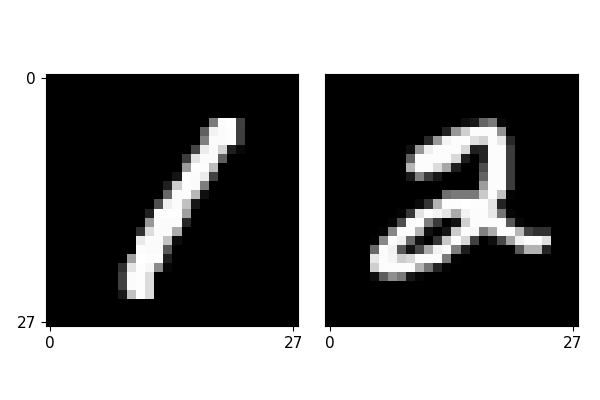
\includegraphics[trim={0cm 1.0cm 0cm 0cm},clip,width=0.95\textwidth]{src/mnist_dataset}
	     \vspace{0.8cm}
	     \end{center}
	\end{column}
    \end{columns}
}

\frame{
    \frametitle{Our experiment}
    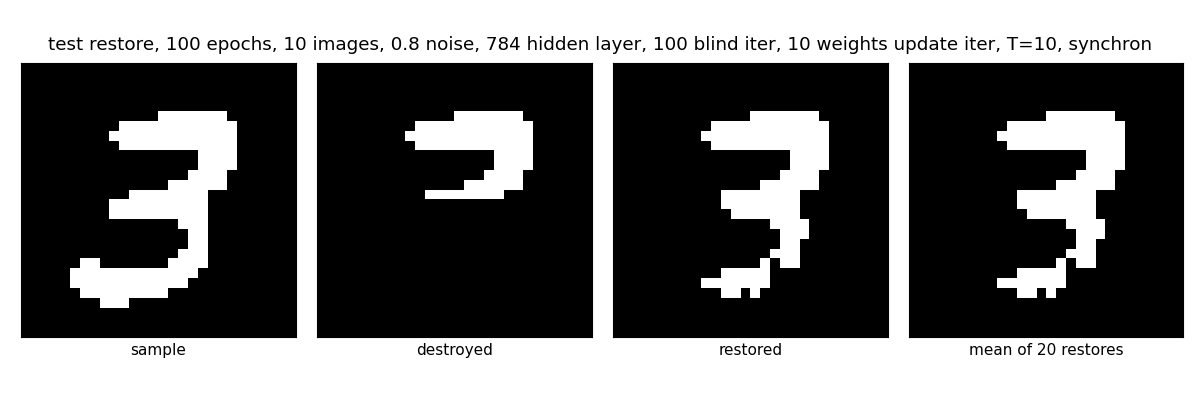
\includegraphics[trim={0cm 1cm 0cm 1.5cm},clip,width=\textwidth]{src/test_restore_10_images}
    \begin{itemize}
        \item Train BM on a subset of images (4$\times$'3', 4$\times$'4', 3$\times$'5')
        \item Take one image, destroy bottom half, let BM restore that
    \end{itemize}
}

\frame{
    \frametitle{Expansion}
    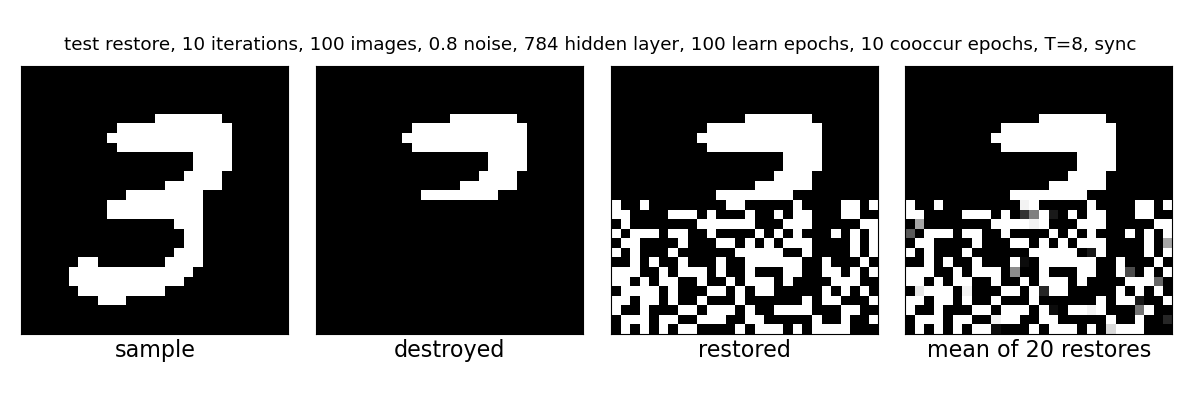
\includegraphics[trim={0cm 1cm 0cm 1.5cm},clip,width=\textwidth]{src/test_restore_100_images}
    \begin{itemize}
        \item Use more images (37$\times$'3', 35$\times$'4', 28$\times$'5')
        \item Although 3's are similar, it seems difficult to recall distribution
    \end{itemize}
}

\frame{
    \frametitle{Tuning number of training epochs}
    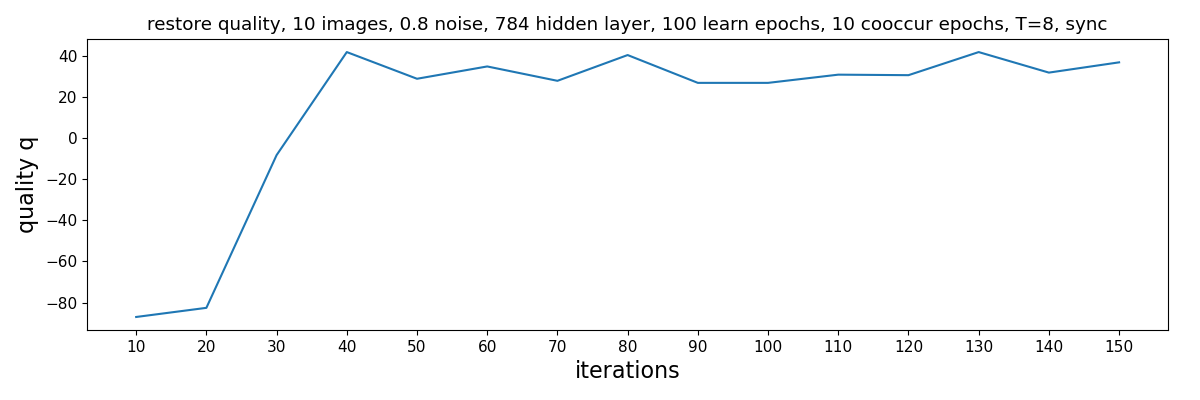
\includegraphics[trim={0.1cm 0.3cm 0cm 0cm},clip,width=\textwidth]{src/test_restore_quality_10_images_vary_epochs}
    \vspace{-5mm}
    \begin{itemize}
        %\item Scan over meta-parameter: Number of training epochs
        \item Very stable convergence for the synchronous update
    \end{itemize}
}

\frame{
    \frametitle{Tuning temperature}
    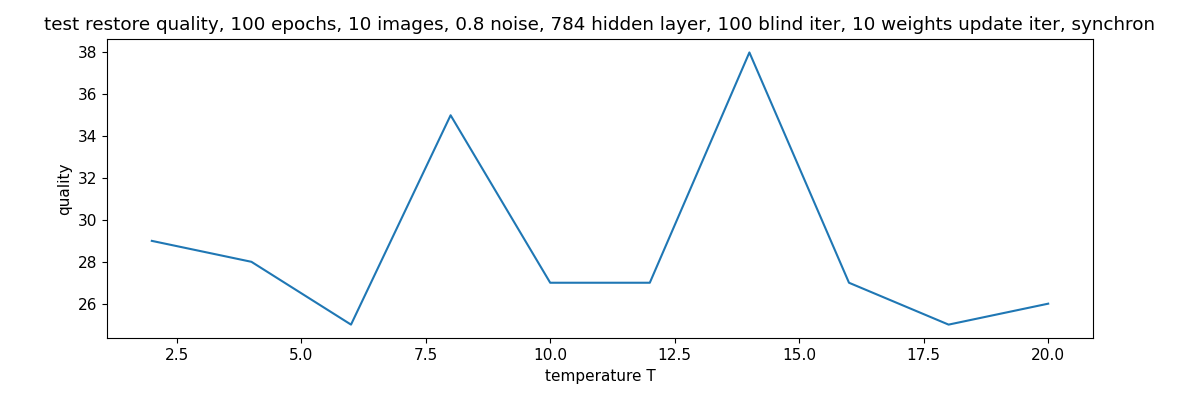
\includegraphics[trim={0.1cm 0.3cm 0.4cm 0cm},clip,width=\textwidth]{src/test_restore_quality_10_images_vary_temperature}
    \vspace{-5mm}
    \begin{itemize}
        %\item Scan over meta-parameter: Temperature
        \item Unstable, very hard to tune this parameter (and others) % could have 2 sentences about conclusion here
    \end{itemize}
}

\frame{
    \frametitle{Future work}
    \begin{itemize}
    	\item Implement with a modern framework (TensorFlow, PyTorch)
    	\item Speed up the computation (GPU computing)
    	\vspace{5mm}
        \item Especially for images: Continuous instead of binary data
        \item Typical use case for recurrent networks: Time series data
    \end{itemize}
}

\section*{}

\frame[c]{
  \frametitle{The End}
\begin{center}
  Thank you for your attention.\\[1ex]
  Any question?\\[2ex]
\end{center}
  \footnotesize
  Literature:
	\begin{itemize}
		\item David H. Ackley, Geoffrey E. Hinton, and Terrence J. Sejnowski. \emph{A Learning Algorithm for Boltzmann Machines}. Cognitive Science, 9(1):147-169, 1985.
		\item Alejandro Cartas. \emph{Boltzmann Machines}, 2014. (accessed 06/2020). \url{http://gorayni.blogspot.com/2014/06/boltzmann-machines.html}.
		\item David JC MacKay. \emph{Information theory, inference and learning algorithms}. Cambridge university press, 2003.
		\item Raul Rojas. \emph{Neural Networks: A Systematic Introduction}. Springer-Verlag, Berlin, Heidelberg, 1996.
	\end{itemize}
}



%%%%%%%%%%%%%%
% TEMPLATE CODE
% \section{Motivation and Question}
%
% \frame[t]{
%   \frametitle{Motivation}
%   \begin{itemize}
%   	\item Add your motivation here
% 		\begin{itemize}
% 			\item Maybe  with some details
% 			\begin{itemize}
% 				\item but not too much
% 			\end{itemize}
% 		\end{itemize}
% 		\item Use references \textsuperscript{[Author, 2010]}
% 	\end{itemize}
% }
%
% \section{Basics and Definition}
%
% \section{Approach}
%
% \section{Results}
%
% \section{Conclusion}
%
% \frame[t]
% {
%   \frametitle{Conclusion}
%
%   Novelty and contribution of this work:
%   \begin{itemize}
% 	  \item Sum up the approach
% 		\item Sum op the results
% 		\item ...
% 		\item Show that it solves the question
%   \end{itemize}
%
% \mbox{ }
%   
% 	Open Questions:
%   \begin{itemize}
%   	\item Something
% 	  \item ... is always missing
%   \end{itemize}
% }
%
% %%%%%%%%%%%%%%
%
% \frame[c]{
%   \frametitle{The End}
% \begin{center}
%   Thank you for your attention.\\[1ex]
%   Any question?\\[5ex]
% \end{center}
%   \footnotesize
%   Literature:
% 	\begin{itemize}
% 		\item Author , Author , Author, and Author. Name of the conference paper. \emph{In: Proceedings of the Conference Name}, 2008
% 		\item Author, Author, and Author. Name of the Article. \emph{Name of the Journal}, 42:111-133, 2010
% 		\item Author, and Author. \emph{Name of the Book}. Publisher, 2009
% 	\end{itemize}
% }

\end{document}
